\section{Adverb}

\begin{table}[h]
	\caption{Adverb characteristics}
	\begin{tabular}{ll}
		\textbf{Title}              & \textbf{Value}      \\
		Semantic value              & Attribute           \\
		Category                    & Independent         \\
		Subcategory                 & Nominal             \\
		Alteration                  & Comparison          \\
		Alteration parameters       & Degree              \\
		Differentiation parameters  & Type, Group
	\end{tabular}
\end{table}

There are different words that cannot be alternated. The biggest class of such words is adverb. It unites a number of groups adverbs can be divided into.

First of all, you should know that adverbs\index{adverb} can be divided into three types, depending on the form they have: \textit{primary} (P), \textit{secondary} (S) and \textit{derivative} (D). When we speak about adverb groups, these letters will be written next to the adverb to help you easier differentiate these types.

\textit{Primary\index{adverb!primary}} adverbs have been formed long ago and we study it as a whole word, without an easy-found root.

\textit{Secondary\index{adverb!secondary}} adverbs have been formed from two words (or a phrase) or from a frozen word form. 

\textit{Derivative\index{adverb!derivative}} adverbs have been shifted semantically from an adjective. It is the most common type of adverbs.

Now let us talk about groups of adverbs. One distinguishes two main types of adverbs: \textit{Significant} and \textit{Demonstrative}. Significant adverbs names concrete property or process attributes, while demonstrative adverbs only refer to these attributes or have an indication of the common nature.

\begin{figure}
	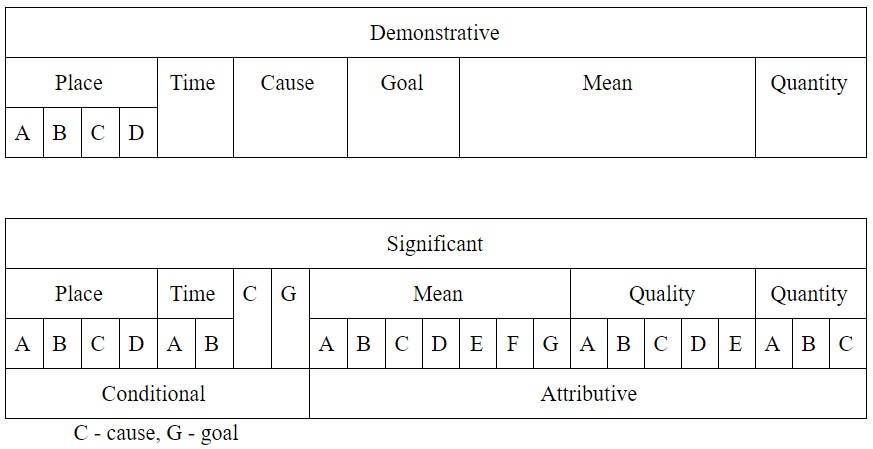
\includegraphics[width=\linewidth]{./sources/adverbs.jpg}
	\caption{Categories of adverbs}
	\label{fig:adverbs}
\end{figure}

\subsection{Demonstrative adverbs}

There are six categories of demonstrative\index{adverb!demonstrative} adverbs. They are adverbs of place, time. cause. goal, mean, quantity.

1. \textbf{Demonstrative adverbs of place.}

Let’s speak about subcategories of this adverbs. 

A. \textit{Adverbs indicating the place of action.}

Question: \textit{Where? (Kųde?)}

Here - \textit{Tut, zdě}

There - \textit{Tamo}

Everywhere - \textit{Vsëde, vsüdu, vsëkųde}

Nowhere - \textit{Nide, nikųde}

Somewhere - \textit{Něde, někųde}

B. \textit{Adverbs indicating the place where action is directed. }

Question: \textit{Whither? (Kųda?)}

Here

There

Everywhere

Nowhere

Somewhere


C. \textit{Adverbs indicating the place of action’s start.}

Question: \textit{Whence? (Odkųde?)}

Here

There

Everywhere

Nowhere

Somewhere


D. \textit{Adverbs indicating the place of action’s start.}

Question: \textit{Where? How far? (Dokųde?)}

(Up to) here

There

Everywhere

Nowhere

Somewhere


2. \textbf{Demonstrative adverbs of time}

Question: \textit{When? (Koĝda?)}

Now

Afterwards

Later

Then

Once

Sometimes

Ever

Never


3. \textbf{Demonstrative adverbs of cause}

Question: \textit{Why? (Čomu?)}

Therefore

Because

Thus

Somehow

Once


4. \textbf{Demonstrative adverbs of goal}

Question: \textit{For what? (Za čto?)}

For

In order to

So as to


5. \textbf{Demonstrative adverbs of mean}

Question: \textit{How? (Kako?)}

So

Likewise

Somehow

Otherwise

Nohow

Like that

That way

Anyhow

Differently


6.\textbf{ Demonstrative adverbs of quantity}

Question: \textit{How much? (Kolïko?)}

So much

Few

Some

Several

Nary


\subsection{Significant adverbs}

Significant\index{adverb!significant} adverbs are often divided into two large subcategories - conditional and attributive adverbs. \textit{Conditional} adverbs shows the conditions of the action took place - place, time, cause, goal. \textit{Attributive} shows the attributes of the action - the mean of the action. its quality and its quantity.

1. \textbf{Significant adverbs of place.}

A. \textit{Adverbs indicating the place of action.}

Question: \textit{Where? (Kųde?)}

Next to (close to)

Ahead

Opposite

Around

Far

Not far

Among

Between

At home

Upstairs

Downstairs


B. \textit{Adverbs indicating the place where action is directed. }

Question:\textit{ Whither? (Kųda?)}

Ahead

To the right

Upwards

Sideways

Downwards

Opposite

Home


C. \textit{Adverbs indicating the place of action’s start.}

Question: \textit{Whence? (Odkųde?)}

From upstairs

From downstairs

From the right

From the left


D. \textit{Adverbs indicating the place of action’s start.}

Question: \textit{Where? How far? (Dokųde?)}

(Up to) here

There

Everywhere

Nowhere

Somewhere


2. \textbf{Significant adverbs of time}

Question: \textit{When? (Koĝda?)}

Now

Afterwards

Later

Then

Once

Sometimes

Ever

Never


3. \textbf{Significant adverbs of cause}

Question: \textit{Why? (Čomu?)}

Therefore

Because

Thus

Somehow

Once


4. \textbf{Significant adverbs of goal}

Question: For what? (Za čto?)

For

In order to

So as to


Further let’s speak about attributive significant pronouns.

1. \textbf{Significant adverbs of mean}

Question: \textit{How? (Kako?)}

So

Likewise

Somehow

Otherwise

Nohow

Like that

That way

Anyhow

Differently

2. \textbf{Significant adverbs of quality}


3.\textbf{ Significant adverbs of quantity}

Question: \textit{How much? (Kolïko?)}

So much

Few

Some

Several

Nary

\subsection{Degrees of comparison}

Likewise adjectives, adverbs have three degrees of comparison\index{comparison}. Moreover, there are synthetic analytic forms too. 

Remember (look at paragraph about adjective degrees of comparison), that there ar three degrees: positive, comparative and superlative.

\textbf{Synthetic forms}

Comparative\index{comparison!synthetic} form is made by adding to the word base the suffix “ěǐ’. Unlike adjectives, this is the only suffix to create a comparative form (compare with suffixes “ëǐ”, “aǐ” for hard and soft bases in adjectives). 

\textbf{Examples:}

\textit{Mnogo - Množěǐ}

\textit{Sïnë - Sïněǐ}

Superlative form is made so as it is in adjectives - adding a suffix “naǐ-” to the comparative form.

\textbf{Analytic forms}

Analytic\index{comparison!analytic} forms provide simple ways of creating comparative and superlative forms without modifying the word itself. There two types of adverb analytic comparison.

\textbf{Using prefixes}

Comparative form is created by adding prefix “po-” through a defis ro a positive form. Superlative form is created by adding prefix “naǐ-” through a defis to the positive form.

\textbf{Examples:}

\textit{Mnogo - po-mnogo - naǐ-mnogo}

\textbf{Using an auxiliary adverb}

To the positive form you should add an auxiliary adverb in comparative or superlative form.

\begin{table}
	\begin{tabular}{lll}
		Auxiliary adverb
		& Comparative form
		& Superlative form \\
		more & bolěǐ & naǐbolěǐ \\
		less & mëněǐ & naǐmëněǐ \\
	\end{tabular}
\end{table}

\textbf{Examples:}

\textit{Mnogo - bolěǐ mnogo - naǐbolěǐ mnogo}

You can use synthetic and analytic forms at the same time.
